\documentclass[a4paper,12pt]{letter}

\usepackage{tikz}
\usepackage{amsmath}
\usepackage{amssymb}
\usepackage{nopageno}
\usepackage[a4paper, total={7.5in, 11.25in}]{geometry}
\usepackage[utf8]{inputenc}
\usepackage[T1]{fontenc}
\usepackage{lmodern}
\usepackage{setspace}
\setstretch{1.2}
\usepackage{pgfplots}
\pgfplotsset{compat=1.18}

\usetikzlibrary{calc,decorations.markings,arrows.meta,patterns}

\begin{document}

\begin{center}
 (KTXFI1EBNF) Physics I. Homework No.~2 Solutions\\ \smallskip
April~20,~2026
\end{center}

\begin{enumerate}

\item We place a copper piece with a mass of 50 gramms and a temperature of $30{}^{\circ}C$ into 250 gramms of water at $90{}^{\circ}C$. What will be the common temperature? The specific heat capacity of copper is $3.85 \cdot 10^{2}\frac{J}{kg\,K}$ and the specific heat capacity of water is $4.19 \cdot 10^{3}\frac{J}{kg\,K}$.

\begin{center}
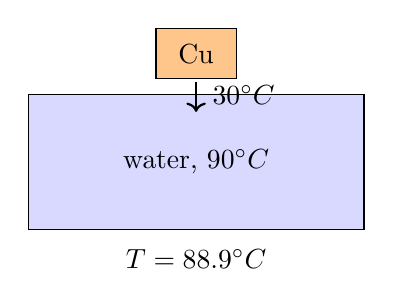
\begin{tikzpicture}[scale=0.85]
\draw[thick] (0,0) rectangle (5,2);
\fill[blue!15] (0,0) rectangle (5,2);
\node at (2.5,1) {water, $90{}^{\circ}C$};
\draw[fill=orange!45] (1.9,2.25) rectangle (3.1,3);
\node at (2.5,2.62) {Cu};
\draw[->,thick] (2.5,2.2) -- (2.5,1.75);
\node[right] at (2.6,2.0) {$30{}^{\circ}C$};
\node at (2.5,-0.45) {$T=88.9{}^{\circ}C$};
\end{tikzpicture}
\end{center}

The heat lost by the water is equal to the heat gained by the copper:
$$m_w c_w(T_w-T)=m_c c_c(T-T_c).$$

Thus
$$T=\frac{m_w c_wT_w+m_c c_cT_c}{m_w c_w+m_c c_c}.$$

Substitution gives
$$T=\frac{m_w c_wT_w+m_c c_cT_c}{m_w c_w+m_c c_c}=\frac{0.250\,\mathrm{kg}\cdot 4.19\cdot 10^3\,\mathrm{\frac{J}{kg\cdot K}}\cdot 90\,\mathrm{K}+0.050\,\mathrm{kg}\cdot 3.85\cdot 10^2\,\mathrm{\frac{J}{kg\cdot K}}\cdot 30\,\mathrm{K}}{0.250\,\mathrm{kg}\cdot 4.19\cdot 10^3\,\mathrm{\frac{J}{kg\cdot K}}+0.050\,\mathrm{kg}\cdot 3.85\cdot 10^2\,\mathrm{\frac{J}{kg\cdot K}}}=362.1\,\mathrm{K}.$$

Therefore
$$\boxed{T=88.9{}^{\circ}C.}$$

% ----------------------------------------------------------------------------------------------------------------------------------

\bigskip

\item At a temperature of $40{}^{\circ}C$, a steel shaft with a diameter of $11.31\,cm$ needs to be fitted with an aluminum ring with an inner diameter of $11.28\,cm$ at the same temperature. The linear thermal expansion coefficient of steel is $12 \cdot 10^{-6}\frac{1}{K}$, and the linear thermal expansion coefficient of alumium is $28.7 \cdot 10^{-6}\frac{1}{K}$. What temperature should the ring be heated to?

\bigskip
  
\begin{center}
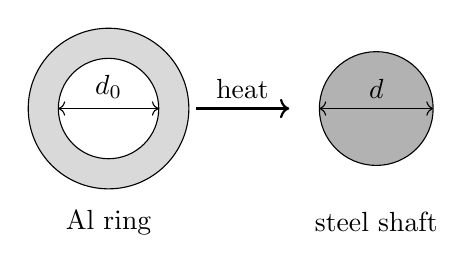
\begin{tikzpicture}[scale=0.85]
\draw[fill=gray!30] (0,0) circle (1.2);
\draw[fill=white] (0,0) circle (0.75);
\node at (0,-1.7) {Al ring};
\draw[<->] (-0.75,0) -- (0.75,0);
\node[above] at (0,0) {$d_{0}$};

\draw[fill=gray!60] (4,0) circle (0.85);
\node at (4,-1.7) {steel shaft};
\draw[<->] (3.15,0) -- (4.85,0);
\node[above] at (4,0) {$d$};

\draw[->,thick] (1.3,0) -- (2.7,0);
\node[above] at (2,0) {heat};
\end{tikzpicture}
\end{center}

The inner diameter of the aluminum ring must expand from $0.1128\,\mathrm{m}$ to $0.1131\,\mathrm{m}$:
$$d=d_0(1+\alpha \Delta T)=\Delta T=\frac{d/d_0-1}{\alpha}=\frac{0.1131\,\mathrm{m}/0.1128\,\mathrm{m}-1}{28.7\cdot 10^{-6}\,\mathrm{1/K}}=92.7\,\mathrm{K}.$$

Hence,
$$T=40{}^{\circ}C+92.7{}^{\circ}C=\boxed{132.7{}^{\circ}C.}$$


% ----------------------------------------------------------------------------------------------------------------------------------

\pagebreak
\item The atmospheric balloon floating at an altitude of several kilometers has a volume of $900\,m^{3}$. The temperature and pressure of the helium inside it are the same as the surrounding $-40{}^{\circ}C$ and $6 \cdot 10^{3}\,Pa$, respectively.
\begin{enumerate}
\item[(a)] How many moles of helium are in the balloon?
\item[(b)] What is the mass of the helium gas? $\left(M = 4 \frac{g}{mol}\right)$
\item[(c)] What was the volume of the balloon at the time of launch on Earth, if the gas inside the balloon was characterized by $0{}^{\circ}C$ and $10^{5}\,Pa$ pressure?
\end{enumerate}

\bigskip

\begin{center}
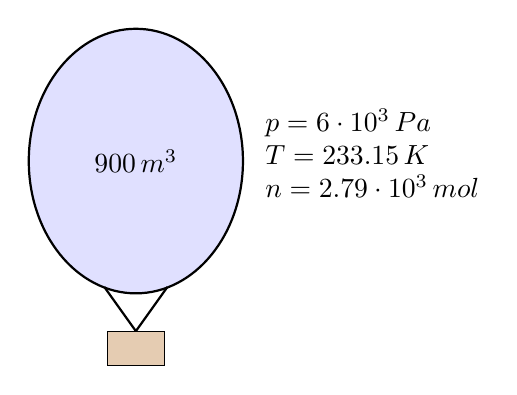
\begin{tikzpicture}[scale=0.8]
\draw[fill=blue!12, thick] (0,0) ellipse (1.7 and 2.1);
\draw[thick] (-0.5,-2) -- (0,-2.7) -- (0.5,-2);
\draw[fill=brown!40] (-0.45,-3.25) rectangle (0.45,-2.7);
\node at (0,0) {$900\,m^3$};
\node[right] at (1.9,0.6) {$p=6\cdot 10^3\,Pa$};
\node[right] at (1.9,0.1) {$T=233.15\,K$};
\node[right] at (1.9,-0.4) {$n=2.79\cdot 10^3\,mol$};
\end{tikzpicture}
\end{center}


The ideal gas law is
$$pV=nRT.$$

Here
$$T=-40{}^{\circ}C=233.15\,K.$$

Therefore
$$n=\frac{pV}{RT}=\frac{6\cdot 10^3\,\mathrm{Pa}\cdot 900\,\mathrm{m^3}}{8.314\,\mathrm{J/K}\cdot 233.15\,\mathrm{K}}=\boxed{2.79\cdot 10^3\,mol.}$$

The mass is
$$m=nM=2.79\cdot 10^3\cdot 4\,g=1.11\cdot 10^4\,g=\boxed{11.1\,kg.}$$

For the launch volume we use
$$\frac{p_1V_1}{T_1}=\frac{p_2V_2}{T_2}.$$

Thus
$$V_1=V_2\frac{p_2}{p_1}\frac{T_1}{T_2}=900\cdot \frac{6\cdot 10^3}{10^5}\cdot \frac{273.15}{233.15}=\boxed{63.3\,m^3.}$$

% ----------------------------------------------------------------------------------------------------------------------------------

\item The ideal cycle of an externally heated heat engine, shown in the diagram, differs from the Otto engine cycle in that it contains isothermal processes instead of adiabatic ones.

\begin{center}
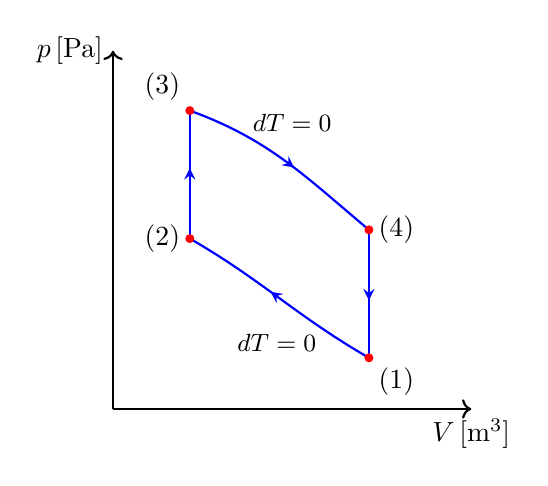
\begin{tikzpicture}[
arrow inside/.style={
postaction={decorate},
decoration={
markings,
mark=at position 0.55 with {\arrow{stealth}}
}
},
scale=0.65]

\draw[thick, ->] (0,0) -- (7,0) node[below] {$V \, [\mathrm{m^3}]$};
\draw[thick, ->] (0,0) -- (0,7) node[left] {$p \, [\mathrm{Pa}]$};

\coordinate (P1) at (5,1);
\coordinate (P2) at (1.5,3.33);
\coordinate (P3) at (1.5,5.83);
\coordinate (P4) at (5,3.5);

\draw[blue, thick, arrow inside] (P1) to[out=150, in=330] (P2);
\draw[blue, thick, arrow inside] (P2) -- (P3);
\draw[blue, thick, arrow inside] (P3) to[out=340, in=140] (P4);
\draw[blue, thick, arrow inside] (P4) -- (P1);

\fill[red] (P1) circle (2.5pt) node[below right, black] {(1)};
\fill[red] (P2) circle (2.5pt) node[left, black] {(2)};
\fill[red] (P3) circle (2.5pt) node[above left, black] {(3)};
\fill[red] (P4) circle (2.5pt) node[right, black] {(4)};

\node[black, font=\small] at (3.2,1.3) {$dT=0$};
\node[black, font=\small] at (3.5,5.6) {$dT=0$};
\end{tikzpicture}
\end{center}

What is the efficiency of the cycle if $p_{3} = 5 p_{2}$, the compression ratio is 6, and the cycle is performed with a two-atomic gas? What is the efficiency of the Carnot cycle taking place between the same temperature limits?

\bigskip

The processes $1\to 2$ and $3\to 4$ are isothermal. The processes $2\to 3$ and $4\to 1$ are isochoric. Since $V_2=V_3$,
$$\frac{T_H}{T_C}=\frac{p_3}{p_2}=5.$$

The compression ratio is
$$r=\frac{V_1}{V_2}=6.$$

For a diatomic gas,
$$C_V=\frac{5}{2}R.$$

The absorbed heat is
$$Q_{in}=nC_V(T_H-T_C)+nRT_H\ln r.$$

Using $T_H=5T_C$,
$$Q_{in}=nR T_C\left(\frac{5}{2}\cdot 4+5\ln 6\right)=nR T_C(10+5\ln 6).$$

The work during the whole cycle is the difference of the two isothermal works:
$$W=nR(T_H-T_C)\ln r=4nRT_C\ln 6.$$

Thus,
$$\eta=\frac{W}{Q_{in}}=\frac{4\ln 6}{10+5\ln 6}=0.378=\boxed{37.8\%.}$$

The Carnot efficiency between the same temperature limits is
$$\eta_C=1-\frac{T_C}{T_H}=1-\frac{1}{5}=0.800=\boxed{80.0\%.}$$

% ----------------------------------------------------------------------------------------------------------------------------------

\item What is the entropy change if the volume of $m = 16\,\mathrm{g}$ of oxygen changes from $V_1 = 20\,\mathrm{l}$ to $V_2 = 80\,\mathrm{l}$, and its temperature changes from $t_1 = 90^\circ\mathrm{C}$ to $t_2 = 300^\circ\mathrm{C}$? The molar mass is $M = 32\,\mathrm{g/mol}$.

\medskip

\begin{center}
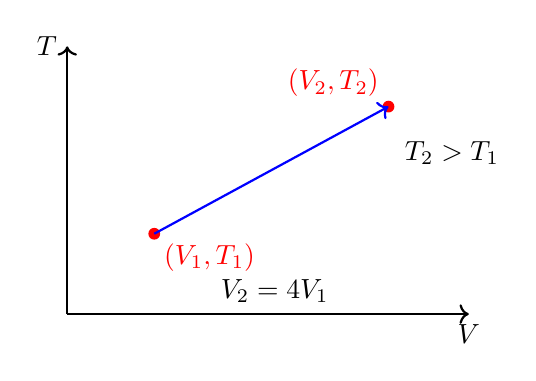
\begin{tikzpicture}[scale=0.85]
\draw[thick,->] (0,0) -- (6,0) node[below] {$V$};
\draw[thick,->] (0,0) -- (0,4) node[left] {$T$};
\fill[red] (1.3,1.2) circle (2.5pt) node[below right] {$(V_1,T_1)$};
\fill[red] (4.8,3.1) circle (2.5pt) node[above left] {$(V_2,T_2)$};
\draw[blue,thick,->] (1.3,1.2) -- (4.8,3.1);
\node at (3.1,0.35) {$V_2=4V_1$};
\node[right] at (4.9,2.4) {$T_2>T_1$};
\end{tikzpicture}
\end{center}

\vskip -20 pt

The amount of substance is
$$n=\frac{m}{M}=\frac{16}{32}=0.5\,mol.$$

The temperatures are
$$T_1=363.15\,K,\qquad T_2=573.15\,K.$$

For an ideal diatomic gas,
$$C_V=\frac{5}{2}R.$$

The entropy change is
$$\Delta S=nC_V\ln\frac{T_2}{T_1}+nR\ln\frac{V_2}{V_1}=0.5\cdot \frac{5}{2}\cdot 8.314\,\mathrm{J/K}\ln\frac{573.15\,\mathrm{K}}{363.15\,\mathrm{K}}+0.5\cdot 8.314\,\mathrm{J/K}\ln\frac{80\,\mathrm{K}}{20\,\mathrm{K}}=\boxed{10.5\,\frac{J}{K}.}$$

\end{enumerate}

\bigskip

\rightline{Dr.~Gabor~FACSKO}
\rightline{\textit{facsko.gabor@uni-obuda.hu}}

\vfill

\end{document}